\documentclass[conference]{IEEEtran}
\IEEEoverridecommandlockouts
% The preceding line is only needed to identify funding in the first footnote. If that is unneeded, please comment it out.
\usepackage{cite}
\usepackage{amsmath,amssymb,amsfonts}
\usepackage{algorithmic}
\usepackage{textcomp}
\usepackage{xcolor}
\usepackage[rightcaption]{sidecap}
\usepackage{wrapfig}
\usepackage{graphicx} %package to manage images
\graphicspath{ {./images/} }


\def\BibTeX{{\rm B\kern-.05em{\sc i\kern-.025em b}\kern-.08em
    T\kern-.1667em\lower.7ex\hbox{E}\kern-.125emX}}
\begin{document}

\title{Sistema de Rega Inteligente}

\author{\IEEEauthorblockN{1\textsuperscript{st} Tomás Marcos}
\IEEEauthorblockA{\textit{Faculdade de Ciências Exatas e da Engenharia} \\
\textit{Universidade da Madeira}\\
Funchal, Portugal \\
2037017@student.uma.pt}
\and
\IEEEauthorblockN{2\textsuperscript{nd} Nelson Vieira}
\IEEEauthorblockA{\textit{Faculdade de Ciências Exatas e da Engenharia} \\
\textit{Universidade da Madeira}\\
Funchal, Portugal \\
2080511@student.uma.pt}
}

\maketitle

\begin{abstract}
A água é um recurso precioso, considerado um dos bens essenciais para a vida. 
No entanto, cada vez mais, ouve-se que é um recurso escasso e que rapidamente está a se esgotar. 
A água é utilizada para muitas atividades, sejam elas industriais, comerciais ou de lazer. 
Existem muitas iniciativas que pretendem reduzir o consumo e o desperdício de água. 
Pretendemos explorar um sistema de rega inteligente que utilize sensores de forma a 
reduzir a quantidade de água que é utilizada. \\
\end{abstract}

\begin{IEEEkeywords}
IoT, Computação ubíqua, Rega inteligente, Análise literária.
\end{IEEEkeywords}

\section{Introdução}
\IEEEPARstart{A} sustentabilidade global não será alcançada sem garantir a 
disponibilidade de água preciosa para todos os consumidores. Apesar de ser um 
dos principais objetivos da agenda da UN2030 para o desenvolvimento global sustentável, 
a atual escassez de água está a crescer rapidamente e afetando um número crescente de consumidores 
de água residencial, comercial, industrial e agrícola em todo o mundo. Espera-se que a procura 
global da água suba 55\%, enquanto atualmente, cerca de 25\% das grandes cidades estão a passar 
por alguns níveis de stress hídrico. 

As mudanças climáticas, secas graves, crescimento populacional, aumento da procura e má 
administração durante as últimas décadas enfatizaram ainda mais os recursos escassos da água 
doce em todo o mundo e resultaram numa grave escassez de água para cerca de 4 bilhões de pessoas, 
pelo menos um mês anualmente. \cite{salehi2022global}

Um dos setores de atividade humana que tem maior consumo dos recursos hídricos é a agricultura, 
"aproximadamente 100 vezes mais do que o uso pessoal é consumida pela alimentação e agricultura 
e quase 70\% das águas fluviais e subterrâneas são utilizadas na irrigação". \cite{nawandar2019iot} 
Várias iniciativas foram tomadas para ajudar a minimizar o desperdício de água neste setor, 
mas, no entanto, não aparentam ter muito sucesso, ou não são apelativas, devido aos 
elevados custos associados. Os sensores comerciais para sistemas destinados à 
agricultura e à sua irrigação são muito caros, tornando impossível aos pequenos 
agricultores a implementação deste tipo de sistema nas suas explorações. 
No entanto, os fabricantes oferecem actualmente sensores de baixo custo que podem 
ser ligados a nós para implementar sistemas de baixo custo para a gestão da 
irrigação e monitorização agrícola. Além disso, devido ao interesse em sensores de 
baixo custo para monitorizar a agricultura e a água, 
novos sensores de baixo custo estão a ser propostos em vários estudos. \cite{garcia2020iot}

Por estes motivos é importante gerir o consumo de água no nosso dia a dia, portanto o que 
propomos é um sistema de rega inteligente que faz a medição da humidade do solo e rega 
as plantas apenas durante o tempo necessário poupando o gasto desnecessário da água de rega.

\section{Trabalhos Relacionados}
Segundo um estudo realizado por García et al, existem 178 artigos relacionados com  
"IoT irrigation, IoT irrigation system, and smart irrigation" \cite{garcia2020iot}, escritos em Inglês, 
no período de entre os anos de 2014 e 2019, inclusive, dos quais 106 artigos estão 
relacionados com a utilização de sensores para monitorizar o estado do solo. 
Destes 106 artigos estudados, todos os artigos abordam a humidade do solo, 
9 discutem a temperatura do solo, 4 exploram o ph do solo e 3 mencionam os 
nutrientes presentes no solo.

Dos artigos que mencionam o tipo de sensor utilizado, o sensor mais popular é o 
e YL69 (SparkFun Electronics, Niwot, CO, USA). Este sensor tem um baixo custo e 
foi criado para operar especificamente com o Arduino. \cite{garcia2020iot}

\subsection{Caso Relacionado}

Muitos sistemas de rega inteligente têm por base sensores de humidade so solo, como 
é o caso do sistema proposto por Goap et al \cite{goap2018an} em que 

\section{Métodos e Metadologias}
O trabalho descrito neste artigo pertende responder a algumas questões que foram 
levantadas após alguma investigação sobre soluções já existentes no que diz respeito 
a sistemas de rega. O sistema proposto permite poupar água? Qual a quantidade de água 
que é possível poupar?  Qual é o custo associado à integração de sensores num sistema 
de rega convencional? Em comparação com um sistema de rega convencional, 
qual a poupança que um sistema de rega inteligente proporciona?

\subsection{O nosso sistema}

O sistema de rega inteligente que propomos faz uso do Arduino MKR 1000 WiFi, de um sensor de 
humidade do solo, modelo 123, de uma breadboard, de vários LEDs e uma resistência de 200 ohms. 
Decidimos usar este modelo do Arduino pela ligação à rede por Wi-fi que possui, o que nos 
permite analisar o sistema sem termos de estar no local da instalação, o que podemos fazer através do 
Arduino Cloud, que envia-nos os resultados do sensor que estamos a usar. Caso o utilizador 
queira ver o estado da humidade do solo, pode perceber pelos LEDs que usamos no sistema, estes 
LEDs mostram um feedback visual do estado atual do solo, decidimos representar este 
feedback com 5 LEDs de várias cores que vão desde o verde até ao vermelho, portanto 
se o LED verde estiver acesso quer dizer que o solo está suficientemente humido, se 
o LED laranja estiver acesso quer dizer que solo requer um pouco de água e se o LED
vermelho estiver acesso quer dizer que o solo está seco, e por isso tem que ser regado.

\begin{figure}
    \centering
    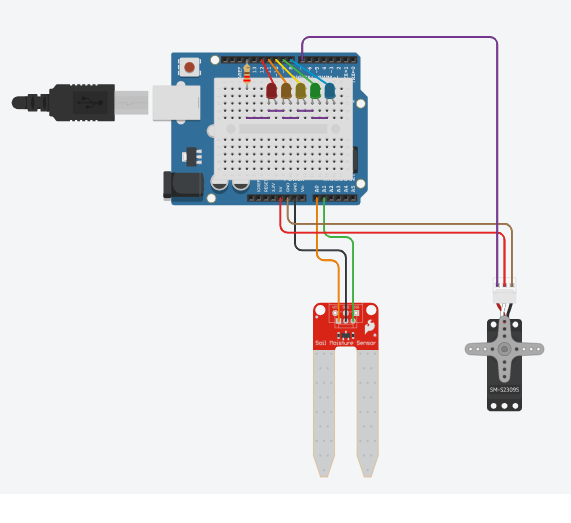
\includegraphics[scale=0.5]{soil_moisture_circuit_schema.png}
    \caption{Dispositivo Arduino}
    \label{fig:my_label1}
\end{figure}

O dispositivo Arduino, como mostra a figura \ref{fig:my_label1}, que usamos é o 
modelo MKR 1000 WiFi pois é um modelo com capacidade wifi, o que facilita na 
transmissão dos dados para o utilizador que poderá vê-los no seu smartphone. 

O sensor de humidade, ilustrado pela figura \ref{fig:my_label1}, é um 
sensor normal para esta função, tem valores de 0 a 1023, serão usados valores 
incrementais entre os valores mínimo e máximo para fazer uma distinção do grau 
de escassez do solo. Também pode ser usado um Raspberry Pi para guardar dados do Arduino.

% END OF ABSTRACT









% \section{Ease of Use}

% \subsection{Maintaining the Integrity of the Specifications}

% \section{Prepare Your Paper Before Styling}

% \subsection{Abbreviations and Acronyms}\label{AA}

% \subsection{Units}
% \begin{itemize}
% \item Use either SI (MKS) or CGS as primary units. (SI units are encouraged.) English units may be used as secondary units (in parentheses). An exception would be the use of English units as identifiers in trade, such as ``3.5-inch disk drive''.
% \item Avoid combining SI and CGS units, such as current in amperes and magnetic field in oersteds. This often leads to confusion because equations do not balance dimensionally. If you must use mixed units, clearly state the units for each quantity that you use in an equation.
% \item Do not mix complete spellings and abbreviations of units: ``Wb/m\textsuperscript{2}'' or ``webers per square meter'', not ``webers/m\textsuperscript{2}''. Spell out units when they appear in text: ``. . . a few henries'', not ``. . . a few H''.
% \item Use a zero before decimal points: ``0.25'', not ``.25''. Use ``cm\textsuperscript{3}'', not ``cc''.)
% \end{itemize}

% \subsection{Equations}

% \begin{equation}
% a+b=\gamma\label{eq}
% \end{equation}

% \subsection{\LaTeX-Specific Advice}


% \subsection{Some Common Mistakes}\label{SCM}
% \begin{itemize}
% \item The word ``data'' is plural, not singular.
% \item The subscript for the permeability of vacuum $\mu_{0}$, and other common scientific constants, is zero with subscript formatting, not a lowercase letter ``o''.
% \item In American English, commas, semicolons, periods, question and exclamation marks are located within quotation marks only when a complete thought or name is cited, such as a title or full quotation. When quotation marks are used, instead of a bold or italic typeface, to highlight a word or phrase, punctuation should appear outside of the quotation marks. A parenthetical phrase or statement at the end of a sentence is punctuated outside of the closing parenthesis (like this). (A parenthetical sentence is punctuated within the parentheses.)
% \item A graph within a graph is an ``inset'', not an ``insert''. The word alternatively is preferred to the word ``alternately'' (unless you really mean something that alternates).
% \item Do not use the word ``essentially'' to mean ``approximately'' or ``effectively''.
% \item In your paper title, if the words ``that uses'' can accurately replace the word ``using'', capitalize the ``u''; if not, keep using lower-cased.
% \item Be aware of the different meanings of the homophones ``affect'' and ``effect'', ``complement'' and ``compliment'', ``discreet'' and ``discrete'', ``principal'' and ``principle''.
% \item Do not confuse ``imply'' and ``infer''.
% \item The prefix ``non'' is not a word; it should be joined to the word it modifies, usually without a hyphen.
% \item There is no period after the ``et'' in the Latin abbreviation ``et al.''.
% \item The abbreviation ``i.e.'' means ``that is'', and the abbreviation ``e.g.'' means ``for example''.
% \end{itemize}
% An excellent style manual for science writers is.

% \subsection{Authors and Affiliations}
% \textbf{The class file is designed for, but not limited to, six authors.} A 
% minimum of one author is required for all conference articles.

% \subsection{Figures and Tables}
% \paragraph{Paragraph} 
% ``Fig.~\ref{fig}''

% \begin{table}[htbp]
% \caption{Table Type Styles}
% \begin{center}
% \begin{tabular}{|c|c|c|c|}
% \hline
% \textbf{Table}&\multicolumn{3}{|c|}{\textbf{Table Column Head}} \\
% \cline{2-4} 
% \textbf{Head} & \textbf{\textit{Table column subhead}}& \textbf{\textit{Subhead}}& \textbf{\textit{Subhead}} \\
% \hline
% copy& More table copy$^{\mathrm{a}}$& &  \\
% \hline
% \multicolumn{4}{l}{$^{\mathrm{a}}$Sample of a Table footnote.}
% \end{tabular}
% \label{tab1}
% \end{center}
% \end{table}

\section{Conclusão}

Um dos maiores problemas que vamos enfrentar num futuro próximo é a escassez de água potável,
e sendo a água um bem essencial para a sobrevivência humana, existe uma preocupação 
em criar sistemas que possibilitem uma melhor gestão da água. Por isto mesmo 
é que proposmos este sistema de rega de água inteligente. Apesar de não ser um 
sistema muito robusto e que pela sua natureza funciona melhor em pequena escala, este 
poderia ser uma ponte para a criação de um sistema mais robusto que funciona-se bem 
tanto áreas pequenas como jardins ou estufas, como também em áreas maiores como campos agrículas.

Para trabalho futuro pode ser integrado um Raspberry Pi neste sistema para uma melhor 
gestão de informação. Um dos pontos fracos que o sistema proposto tem é não 
ter em conta a previsão do tempo o que pode tornar este sistema menos eficiente, 
portanto ter uma previsão...

\section*{Acknowledgment}

Gostaria de agradecer a todas as pessoas que me apoiaram até agora, incluindo
família, amigos e professores.

\bibliographystyle{IEEEtran}
\bibliography{references}

\end{document}
